\documentclass[12pt]{article}

\usepackage{sbc-template}
\usepackage{graphicx,url}
\usepackage[utf8]{inputenc}
\usepackage[brazil]{babel}
\usepackage{amsmath,amssymb}
\usepackage{booktabs}

\sloppy

\title{Análise Empírica e Otimização para o Problema do Caixeiro Viajante}

\author{Joseph Patrick Alves de Moura}

\address{Departamento de Ciência da Computação -- Universidade Federal de Minas Gerais (UFMG)\\
  Belo Horizonte -- MG -- Brasil
  \email{josephmoura@ufmg.br}
}

\begin{document} 

\maketitle

\begin{abstract}
  This paper presents an empirical comparison, subroutine profiling, and implementation audit of exact and approximation algorithms for the Traveling Salesman Problem (TSP) evaluated across 12 TSPLIB instances. We contrast a Branch-and-Bound (B\&B) solver with two classical approximation algorithms: Twice-around-the-tree (TAT) and Christofides (CHR). Across 253 experimental runs, both heuristics solved all instances within milliseconds (median gaps of 7.05\% for CHR and 29.25\% for TAT), whereas the exact B\&B solver hit the 1800~s timeout in 91 runs, collapsing beyond $N\geq22$ regardless of the initialization strategy. Subroutine profiling reveals that minimum-weight matching accounts for up to 95.10\% of CHR's runtime, Prim's MST accounts for 88.47\%--95.55\% of TAT, and matrix reduction consumes roughly 59\%--67\% of B\&B's search time. Finally, we audit memory instrumentation biases (\texttt{tracemalloc}) and show that integer rounding in TSPLIB introduces triangle inequality violations even in Euclidean instances.
\end{abstract}
     
\begin{resumo} 
  Este trabalho apresenta uma comparação empírica, análise de profiling por subrotina e auditoria de implementação de algoritmos exatos e aproximativos para o Problema do Caixeiro Viajante (TSP) avaliados em 12 instâncias da TSPLIB. Contrastamos um resolvedor exato baseado em Branch-and-Bound (B\&B) com dois algoritmos exatos clássicos: Twice-around-the-tree (TAT) e Christofides (CHR). Ao longo de 253 execuções, ambas as heurísticas concluíram todas as instâncias em milissegundos (gaps medianos de 7,05\% para o CHR e 29,25\% para o TAT), enquanto o B\&B atingiu o limite de 1800~s em 91 execuções, colapsando a partir de $N\geq22$ independentemente da estratégia de inicialização. O profiling por subrotina revela que o emparelhamento mínimo concentra até 95,10\% do tempo do CHR, a MST de Prim responde por 88,47\%--95,55\% do TAT e a redução de matriz absorve cerca de 59\%--67\% do tempo de busca do B\&B. Por fim, auditamos vieses da medição de memória (\texttt{tracemalloc}) e mostramos que o arredondamento inteiro da TSPLIB introduz violações da desigualdade triangular mesmo em instâncias euclidianas.
\end{resumo}

\section{Introdução}

O Problema do Caixeiro Viajante (TSP, do inglês \textit{Traveling Salesman Problem}) consiste em determinar um circuito hamiltoniano de custo mínimo que visite cada um dos $N$ vértices de um grafo ponderado completo exatamente uma vez, retornando à origem. Por pertencer à classe NP-difícil, não se conhece um algoritmo capaz de resolvê-lo exatamente em tempo polinomial no pior caso. Em razão desta barreira computacional, algoritmos exatos e aproximativos são estudados de forma complementar: os métodos exatos asseguram a otimalidade global ao custo de uma exploração potencialmente exponencial, enquanto os algoritmos aproximativos operam em tempo polinomial, oferecendo limitantes teóricos para a razão entre o custo obtido e o ótimo.

Este trabalho compara, usando um conjunto de $12$ instâncias da biblioteca TSPLIB, um algoritmo exato baseado em \textit{Branch-and-Bound} (B\&B) e dois algoritmos aproximativos: \textit{Twice-around-the-tree} (TAT), com fator de aproximação $2$, e o algoritmo de Christofides (CHR), com fator $1{,}5$. O estudo foca na auditoria das implementações, na avaliação do impacto de cinco estratégias de inicialização do limite superior (\textit{warm-start}) sobre a poda da árvore de busca e na investigação de como propriedades geométricas e violações métricas afetam a qualidade das aproximações. A investigação se baseia em três eixos:
\begin{enumerate}
    \item \textbf{Complexidade assintótica versus comportamento empírico:} avaliando como os limites teóricos se comportam nas amostras observadas.
    \item \textbf{Efetividade do \textit{warm-start} na poda:} a inicialização heurística do limite superior (\textit{upper bound}, UB) apenas reduz o esforço de busca do B\&B quando estabelece um teto estritamente menor que o primeiro custo encontrado.
    \item \textbf{Restrições métricas nas garantias aproximativas:} os fatores teóricos $2$ e $1{,}5$ pressupõem a validade da desigualdade triangular. Como o conjunto experimental abrange instâncias explícitas e funções de distância com arredondamento inteiro da TSPLIB que violam essa condição, torna-se indispensável separar os efeitos de arredondamento e avaliar seu reflexo nos \textit{gaps} empíricos.
\end{enumerate}

\section{Implementação, Profiling e Auditoria}

A arquitetura do sistema foi estruturada em Python~3 de forma modular, separando o núcleo algorítmico (\texttt{aproximativos.py} e \texttt{branch\_bound.py}), a extração de características geométricas (\texttt{features.py}), os geradores de experimentos (\texttt{harness.py} e \texttt{worker.py}) e a modelagem estatística e análises dos resultados(\texttt{regressao.py}).

\subsection{Representação das Instâncias e Cálculo de Distâncias}

Cada instância no formato TSPLIB é lida uma única vez na etapa de inicialização (\texttt{ler\_tsplib}) e convertida em uma matriz densa de custos inteiros $D \in \mathbb{Z}^{N \times N}$ (\texttt{construir\_matriz}). Para instâncias baseadas em coordenadas bidimensionais, aplicam-se as especificações oficiais da TSPLIB:
\begin{itemize}
    \item \texttt{EUC\_2D} e \texttt{CEIL\_2D}: distância euclidiana vetorizada via NumPy, seguida, respectivamente, pelo arredondamento ao inteiro mais próximo ($\lfloor d + 0{,}5 \rfloor$) e pela função teto ($\lceil d \rceil$).
    \item \texttt{GEO}: conversão das coordenadas de graus e minutos para radianos e cálculo da distância geodésica sobre o globo terrestre ($R = 6378{,}388\text{ km}$).
    \item \texttt{ATT}: métrica pseudo-euclidiana com fator de escala $\sqrt{(\Delta x^2 + \Delta y^2)/10}$ e regra específica de arredondamento da biblioteca.
    \item \texttt{EXPLICIT}: leitura e expansão direta das matrizes simétricas fornecidas no arquivo (suportando os formatos \texttt{FULL\_MATRIX}, \texttt{UPPER\_ROW}, \texttt{LOWER\_ROW}, \texttt{UPPER\_DIAG\_ROW} e \texttt{LOWER\_DIAG\_ROW}).
\end{itemize}

Todos os algoritmos e heurísticas operam sobre exatamente a mesma matriz $D$, e todos os custos e \textit{gaps} relativos são recalculados sobre ela. Os valores ótimos publicados no site da TSPLIB atuam como referência externa de avaliação, nunca sendo passados como entrada.

\subsection{Twice-around-the-tree e Christofides}

Ambos os algoritmos iniciam criando uma Árvore Geradora Mínima (MST) utilizando o algoritmo de Prim (\texttt{prim\_mst}). Como o TSP é definido sobre um grafo completo denso ($|E| = \mathcal{O}(N^2)$), optou-se pela implementação baseada em vetores lineares com seleção do mínimo via NumPy, conseguindo a complexidade $\mathcal{O}(N^2)$. Uma implementação apoiada em fila de prioridades (utilizando um \textit{heap}) poderia ter um custo $\mathcal{O}(N^2 \log N)$ por conta de sucessivas atualizações de chaves nos grafos densos, tornando a abordagem vetorial mais adequada.

No algoritmo \textit{Twice-around-the-tree}, a lista de adjacência da MST é ordenada lexicograficamente e percorrida em pré-ordem por meio de uma pilha explícita (\texttt{dfs\_pre\_ordem}), evitando os limites de profundidade de recursão do interpretador Python. A aplicação de atalhos (\textit{shortcutting}) ocorre implicitamente ao registrar apenas a primeira ocorrência de cada vértice durante a travessia.

No algoritmo de Christofides, identificam-se os vértices de grau ímpar na MST e constrói-se o subgrafo completo induzido sobre eles. O emparelhamento perfeito de custo mínimo é obtido pela função \texttt{min\_weight\_matching} da biblioteca NetworkX, passando os pesos inteiros originais de $D$. As arestas da MST e do emparelhamento são reunidas em uma lista de multigrafo e percorridas pelo algoritmo de Hierholzer implementado de forma iterativa com pilha explícita e identificadores únicos por aresta (\texttt{circuito\_euleriano}). Por fim, o circuito euleriano é convertido em ciclo hamiltoniano pela remoção de vértices repetidos (\texttt{atalhos}).

Em ambos os algoritmos, o circuito final é submetido a uma rotina independente de auditoria (\texttt{validar\_e\_custo}), que verifica se o vetor resultante constitui uma permutação válida de $\{0, \dots, N-1\}$ e recalcula o custo fechado diretamente sobre $D$.

\subsection{Branch-and-Bound e Estratégias de Warm-Start}

O resolvedor exato (\texttt{branch\_and\_bound}) implementa o esquema de redução de matrizes de Little et al. . Em cada nó da árvore de busca, constrói-se uma cópia da matriz residual (\texttt{construir\_matriz\_residual}) bloqueando (com valor sentinela $\text{INF} = 10^{12}$) a diagonal principal, as linhas dos vértices já deixados no caminho parcial, as colunas dos vértices já alcançados e o retorno prematuro ao vértice inicial $0$ enquanto o caminho possui menos que $N$ vértices. O limite inferior (\textit{lower bound}, LB) é obtido somando o custo real das arestas já fixadas ao total subtraído na redução mínima de linhas e colunas da submatriz aberta (\texttt{matriz\_reducao}).

A exploração da árvore é conduzida em profundidade por meio de uma pilha explícita. Ao expandir um nó (\texttt{expansao\_no}), os filhos viáveis são gerados, avaliados e ordenados em ordem crescente de LB, garantindo que o filho mais promissor (menor LB) seja explorado primeiro. Qualquer filho com $\text{LB} \ge \text{UB}$ é imediatamente podado, nunca passando pela pilha.

Antes do início da busca, o limite superior inicial ($\text{UB}$) é definido por uma das cinco estratégias de \textit{warm-start}:
\begin{enumerate}
    \item \textbf{Cold Start / Trivial:} solução sequencial/ingênua $(0, 1, 2, \dots, N-1, 0)$.
    \item \textbf{Vizinho Mais Próximo:} construção gulosa partindo sempre do vértice $0$ (\texttt{vizinho\_mais\_proximo}).
    \item \textbf{Inserção pelo Fecho Convexo:} determinação da envoltória convexa pelo algoritmo \textit{monotone chain} de Andrew (\texttt{fecho\_convexo}) seguida da inserção incremental gulosa de menor custo (\texttt{insercao\_feixo}). Para instâncias do tipo \texttt{EXPLICIT}, nas quais não há coordenadas geométricas, a estratégia é marcada como não aplicável (\texttt{nao\_aplicavel}).
    \item \textbf{Twice-around-the-tree (TAT):} custo do circuito gerado pela heurística TAT.
    \item \textbf{Christofides (CHR):} custo do circuito gerado pelo algoritmo de Christofides.
\end{enumerate}
Todas as estratégias garantem a convergência para o mesmo ótimo global quando concluídas dentro do tempo limite, alterando exclusivamente a trajetória de poda e o número de nós expandidos.

Foi escolhida a busca em profundidade (DFS) em vez da busca pelo melhor primeiro (\textit{best-first search}) por três motivos: (i) consumo de memória linear na profundidade da árvore ($\mathcal{O}(N)$ estados ativos na pilha), evitando o acúmulo exponencial de fronteiras abertas e cópias de matrizes; (ii) disponibilidade imediata de limites superiores competitivos fornecidos pelo \textit{warm-start}, reduzindo a necessidade de encontrar soluções viáveis rapidamente pela busca; e (iii) maior previsibilidade e controle sobre a alocação de memória durante execuções prolongadas.

\subsection{Protocolo de Medição, Profiling e Controle de Execução}

O ambiente experimental (\texttt{harness.py} e \texttt{worker.py}) foi projetado para eliminar interferências de instrumentação e garantir reprodutibilidade:

\begin{itemize}
    \item \textbf{Segregação entre tempo e memória:} os primeiros testes feitos mostraram que a ativação do módulo \texttt{tracemalloc} do Python eleva o tempo de execução em aproximadamente $5\times$ a $6\times$. Por isso, cada combinação experimental é executada em dois modos distintos: no modo \texttt{tempo} (com paralelismo desabilitado por padrão para evitar contenção de CPU), o rastreamento de memória permanece desligado; no modo \texttt{memoria}, o \texttt{tracemalloc} é ativado para registrar o pico de alocação em megabytes, utilizando chamadas a \texttt{tracemalloc.reset\_peak()} por sub-rotina nos algoritmos aproximativas e monitoramento global de pico de pilha no B\&B.
    \item \textbf{Isolamento de processos e duplo \textit{timeout}:} cada execução ocorre em um subprocesso independente do sistema operacional. Um temporizador interno verifica o tempo decorrido a cada iteração da pilha do B\&B; ao atingir $1800\text{ s}$ ($30\text{ min}$), a busca é interrompida, preservando os contadores parciais de nós expandidos, nós podados, profundidade máxima e o menor LB remanescente na pilha, marcando o status como \texttt{NA} (\texttt{motivo\_NA = timeout}). Na análise estatística, execuções interrompidas são tratadas como censura à direita, e não como falhas de código.
    \item \textbf{Hierarquia de \textit{profiling}:} no TAT e CHR, as subrotinas (\texttt{prim\_mst}, \texttt{grau\_mst}, \texttt{emparelhamento}, \texttt{euler}, \texttt{atalhos} e \texttt{validar\_e\_custo}) são sequenciais e disjuntas, permitindo somar seus tempos para compor o custo total. No B\&B, as rotinas são hierarquicamente aninhadas (\texttt{matriz\_reducao} ocorre dentro de \texttt{calculo\_lb}, que se junta a \texttt{expansao\_no}, localizada em \texttt{busca\_total}); por conta disso, seus tempos são reportados como frações percentuais relativas a \texttt{busca\_total}, sem soma direta.
\end{itemize}

\subsection{Auditoria e Refatorações Realizadas}

Ferramentas de inteligência artificial generativa auxiliaram na escrita inicial dos módulos, com os prompts preservado nos anexos do repositório. A auditoria técnica sobre o código bruto gerado identificou pequenas falhas que necessitaram de intervenção antes da coleta dos resultados:

\begin{enumerate}
    \item \textbf{Separação de violações da desigualdade triangular:} verificou-se que o arredondamento inteiro da TSPLIB pode induzir violações métricas em instâncias originalmente euclidianas. Logo, incluiu-se a auditoria (\texttt{obter\_violacoes}) para contabilizar separadamente as triplas $(i, j, k)$ que violam $D_{ij} > D_{ik} + D_{kj}$ nas distâncias contínuas em ponto flutuante (\texttt{violacoes\_reais}, aplicável a \texttt{EUC\_2D} e \texttt{CEIL\_2D}) e na matriz inteira final $D$ (\texttt{violacoes\_arredondadas}).
    \item \textbf{Isolamento do pico de memória entre subrotinas:} na implementação inicial das heurísticas, o pico reportado pelo \texttt{tracemalloc} acumulava o máximo global desde o início do script. A inserção de \texttt{tracemalloc.reset\_peak()} na entrada do gerenciador de contexto \texttt{medir()} isolou o consumo real de cada subrotina.
    \item \textbf{Desacoplamento de modos de execução:} a criação explícita dos parâmetros \texttt{--modo tempo} e \texttt{--modo memoria} no \textit{harness} eliminou a distorção de $5\times$ a $6\times$ nos tempos causada pela instrumentação de memória.
    \item \textbf{Validação exaustiva contra força bruta:} a corretude do B\&B e das cinco estratégias de \textit{warm-start} foi auditada em \texttt{validar\_forca\_bruta}, confrontando o resolvedor com uma enumeração exaustiva (\texttt{itertools.permutations}) em $50$ instâncias sintéticas aleatórias com $4 \le N \le 9$, confirmando $100\%$ de concordância nos custos ótimos e invariância entre estratégias.
    \item \textbf{Teste de controle de poda no B\&B:} para comprovar que o limite superior atua efetivamente na redução da árvore, executou-se um controle na instância \texttt{burma14} inicializando o $\text{UB}$ diretamente com o ótimo conhecido ($3323$). Observou-se uma redução de $30{,}6\%$ no número de nós expandidos em relação à estratégia \texttt{trivial}, validando o mecanismo de poda.
    \item \textbf{Testes preliminares em instâncias de referência:} antes da bateria experimental completa, foram executados testes controlados nas instâncias \texttt{burma14} ($N=14$, tipo \texttt{GEO}) e \texttt{gr17} ($N=17$, tipo \texttt{EXPLICIT}). No B\&B, verificou-se que todas as estratégias de inicialização (\textit{warm-start}) convergiam para os ótimos publicados na literatura ($3323$ e $2085$, respectivamente), enquanto nos algoritmos aproximativos confirmou-se o cumprimento dos limitantes teóricos de aproximação ($2 \times \text{OPT}$ e $1{,}5 \times \text{OPT}$).
\end{enumerate}

\section{Experimentos e Resultados}

Esta seção apresenta a configuração experimental e a análise empírica dos algoritmos exato e aproximativos, cobrindo o ajuste de curvas de complexidade, a eficiência de expansão e poda sob diferentes estratégias de inicialização (\textit{warm-start}), a qualidade das aproximações, a sensibilidade às características geométricas das instâncias e o \textit{profiling} de subrotinas.

\subsection{Instâncias, Configuração e Ambiente Computacional}

O conjunto experimental é composto por $12$ instâncias da biblioteca TSPLIB, detalhadas na Tabela~\ref{tab:instancias}. Desse total, $9$ instâncias ($75\%$) situam-se na faixa principal ($N \le 40$) e $3$ ($25\%$) na faixa de estresse ($41 \le N \le 75$).

Embora o enunciado mencione instâncias do tipo \texttt{EUC\_2D}, o conjunto avaliado incorpora instâncias dos tipos \texttt{GEO} (\texttt{burma14}, \texttt{ulysses16}, \texttt{ulysses22}), \texttt{ATT} (\texttt{att48}) e \texttt{EXPLICIT} (\texttt{gr17}, \texttt{gr21}, \texttt{gr24}, \texttt{fri26}, \texttt{bayg29}, \texttt{bays29}), conforme autorizado pelo professor, permitindo o uso de qualquer instância da biblioteca cuja função de custo represente uma distância. Como os limitantes teóricos de aproximação ($2$ para TAT e $1{,}5$ para CHR) exigem a validade da desigualdade triangular, as violações métricas decorrentes da definição explícita ou do arredondamento inteiro são auditadas na Seção~\ref{sec:violacoes}. Os ótimos publicados na Tabela~\ref{tab:instancias} foram conferidos junto à documentação oficial da TSPLIB e servem somente como referência externa.

\begin{table}[ht]
\centering
\caption{Conjunto experimental de instâncias da TSPLIB, tipo de função de custo, ótimo publicado e faixa de tamanho.}
\label{tab:instancias}
\small
\begin{tabular}{lcccc}
\toprule
\textbf{Instância} & \textbf{$N$} & \textbf{Tipo de Distância} & \textbf{Ótimo} & \textbf{Grupo ($N$)} \\
\midrule
\texttt{burma14}   & 14 & \texttt{GEO}      & 3323  & $\le 40$ \\
\texttt{ulysses16} & 16 & \texttt{GEO}      & 6859  & $\le 40$ \\
\texttt{gr17}      & 17 & \texttt{EXPLICIT} & 2085  & $\le 40$ \\
\texttt{gr21}      & 21 & \texttt{EXPLICIT} & 2707  & $\le 40$ \\
\texttt{ulysses22} & 22 & \texttt{GEO}      & 7013  & $\le 40$ \\
\texttt{gr24}      & 24 & \texttt{EXPLICIT} & 1272  & $\le 40$ \\
\texttt{fri26}     & 26 & \texttt{EXPLICIT} & 937   & $\le 40$ \\
\texttt{bayg29}    & 29 & \texttt{EXPLICIT} & 1610  & $\le 40$ \\
\texttt{bays29}    & 29 & \texttt{EXPLICIT} & 2020  & $\le 40$ \\
\texttt{att48}     & 48 & \texttt{ATT}      & 10628 & $41$--$75$ \\
\texttt{berlin52}  & 52 & \texttt{EUC\_2D}  & 7542  & $41$--$75$ \\
\texttt{st70}      & 70 & \texttt{EUC\_2D}  & 675   & $41$--$75$ \\
\bottomrule
\end{tabular}
\end{table}

\paragraph{Protocolo de Coleta e Ambiente.} Foram registradas $253$ execuções no total, divididas em $144$ concluídas com sucesso (\texttt{OK}), $91$ interrompidas por atingirem o limite de $1800\text{ s}$ (\texttt{timeout}) e $18$ classificadas como não aplicáveis (\texttt{nao\_aplicavel}), correspondentes à heurística de fecho convexo sobre as $6$ matrizes \texttt{EXPLICIT} desprovidas de coordenadas. Ressalta-se que \texttt{timeout} e \texttt{nao\_aplicavel} constituem categorias metodológicas distintas e não foram agrupadas. No modo de medição de tempo, aplicaram-se $3$ repetições para instâncias com $N \le 22$ e $1$ repetições para as demais, adotando-se a mediana como estimador central; ressalta-se que repetições medem variabilidade operacional e não ampliam o tamanho amostral de instâncias independentes. Para o modo de memória, executou-se $1$ repetição por configuração, partindo-se da premissa de determinismo nas alocações de memória monitoradas pelo \texttt{tracemalloc}. As heurísticas TAT e CHR concluíram $100\%$ das execuções previstas, enquanto as interrupções por tempo concentraram-se integralmente no B\&B ($55$ no modo tempo e $36$ no modo memória).

Os experimentos foram executados de forma sequencial (\texttt{workers=1}) em ambientes distintos entre modos: as medições de tempo foram coletadas em uma estação Windows~11 equipada com processador AMD64 Family 23 Model 104 Stepping 1 ($8$ núcleos físicos, $16$ lógicos), $31{,}39\text{ GB}$ de RAM, Python~$3.13.1$, NumPy~$2.3.5$ e NetworkX~$3.7$; já as medições de memória foram coletadas em duas máquinas Intel (Windows~11, Intel64 Family 6 Model 126 Stepping 5, $2$ núcleos físicos / $4$ lógicos, $15{,}75\text{ GB}$ de RAM; e Windows~10, Intel64 Family 6 Model 60 Stepping 3, $4$ núcleos físicos / $8$ lógicos, $15{,}92\text{ GB}$ de RAM), ambas com Python~$3.15.2$, NumPy~$2.5.5$ e NetworkX~$3.7$. Em razão dessa diferença de \textit{hardware}, os modos de tempo e memória são analisados de forma isolada.


\subsection{Complexidade Empírica e Censura}

Para explorar tendências de crescimento em função do número de vértices $N$, ajustaram-se curvas paramétricas da forma $y = a \cdot f(N) + b$, com $f(N) \in \{N, N^2, N^3, N \log N\}$, avaliando o coeficiente de determinação ($R^2$) e a raiz do erro quadrático médio (RMSE) na escala original dos dados. Como o tamanho amostral varia entre $4$ e $12$ instâncias distintas, múltiplos modelos produzem ajustes numericamente próximos; portanto, apresentam-se todos os modelos candidatos sem eleger um único como prova de classe de complexidade assintótica.

\begin{table}[ht]
\centering
\caption{Coeficiente de determinação ($R^2$ na escala original) dos modelos empíricos para tempo total e pico de memória dos algoritmos aproximativos ($n = 12$ instâncias).}
\label{tab:regressao_aprox}
\small
\begin{tabular}{llcccc}
\toprule
\textbf{Série} & \textbf{Métrica} & \textbf{$N$} & \textbf{$N^2$} & \textbf{$N^3$} & \textbf{$N \log N$} \\
\midrule
TAT & Tempo total (s)   & 0,3791 & 0,2994 & 0,2246 & 0,3632 \\
CHR & Tempo total (s)   & 0,8121 & 0,8208 & 0,7905 & 0,8189 \\
\midrule
TAT & Memória pico (MB) & 0,9851 & 0,9111 & 0,8119 & 0,9735 \\
CHR & Memória pico (MB) & 0,9957 & 0,9637 & 0,8918 & 0,9944 \\
\bottomrule
\end{tabular}
\end{table}

Conforme mostrado na Tabela~\ref{tab:regressao_aprox}, os tempos de execução do TAT apresentam baixa correlação com $N$ ($R^2 \le 0{,}3791$), refletindo o fato de que durações na faixa de décimos de milissegundo ($0{,}4\text{ ms}$ a $1{,}8\text{ ms}$) sofrem forte influência da sobrecarga fixa do interpretador Python e da resolução de escalonamento do sistema operacional. No algoritmo de Christofides, o crescimento de tempo acompanha mais de perto o aumento de $N$ ($R^2 = 0{,}8208$ para o modelo quadrático e $0{,}8189$ para $N \log N$), impulsionado pelo custo do emparelhamento em grafos maiores. No modo memória, ambos exibem ajustes elevados para modelos lineares e $N \log N$ ($R^2 > 0{,}97$), mas esses valores refletem apenas alocações de listas e estruturas auxiliares em Python capturadas pelo \texttt{tracemalloc} (Seção~\ref{sec:violacoes}).

No algoritmo exato B\&B, o comportamento empírico é governado pela estrutura combinatória da instância e pela censura por \textit{timeout}:
\begin{itemize}
    \item \textbf{Tempo de execução e nós expandidos:} Considerando as $4$ instâncias concluídas pelas estratégias \texttt{trivial}, \texttt{vizinho}, \texttt{TAT} e \texttt{CHR} (\texttt{burma14}, \texttt{ulysses16}, \texttt{gr17} e \texttt{gr21}), todos os modelos em função de $N$ exibem $R^2$ nulo ou desprezível, situando-se entre $0{,}0021$ e $0{,}0257$ para o tempo total e entre $0{,}0082$ e $0{,}0409$ para nós expandidos. Isso ocorre porque o esforço computacional não cresce monotonicamente com $N$: a instância \texttt{gr17} ($N=17$) expandiu $406.037$ nós ($147{,}19\text{ s}$ na estratégia \texttt{trivial}), enquanto \texttt{gr21} ($N=21$) exigiu apenas $21.715$ nós ($12{,}81\text{ s}$). Para a estratégia \texttt{fecho}, apenas $2$ instâncias foram concluídas, inviabilizando qualquer regressão.
    \item \textbf{Memória e efeito de censura:} Embora os ajustes de pico de memória do B\&B sobre os $4$ pontos concluídos exibam $R^2$ entre $0{,}9873$ e $0{,}9998$, o resultado deve ser levado com cautela devido a pequena quantidade de amostras. Mais criticamente, as $55$ interrupções no modo tempo e $36$ no modo memória ($8$ instâncias estouradas para \texttt{trivial}, \texttt{vizinho}, \texttt{TAT} e \texttt{CHR}, e $4$ para \texttt{fecho}) mostram que as instâncias mais difíceis são justamente as excluídas das curvas ajustadas, fazendo com que qualquer regressão sobre os casos concluídos subestime severamente o crescimento real do algoritmo exato.
\end{itemize}

\begin{table}[ht]
\centering
\caption{Distribuição das $253$ execuções por algoritmo, estratégia de \textit{warm-start} e modo de medição (\texttt{OK} / \texttt{timeout} / \texttt{nao\_aplicavel}).}
\label{tab:status_execucoes}
\small
\begin{tabular}{llccc}
\toprule
\textbf{Algoritmo} & \textbf{Estratégia} & \textbf{Modo Tempo} & \textbf{Modo Memória} & \textbf{Instâncias Concluídas} \\
\midrule
B\&B & \texttt{trivial} & 12 \texttt{OK} / 13 \texttt{TO} & 4 \texttt{OK} / 8 \texttt{TO} & \texttt{burma14}, \texttt{ulysses16}, \texttt{gr17}, \texttt{gr21} \\
B\&B & \texttt{vizinho} & 12 \texttt{OK} / 11 \texttt{TO} & 4 \texttt{OK} / 8 \texttt{TO} & \texttt{burma14}, \texttt{ulysses16}, \texttt{gr17}, \texttt{gr21} \\
B\&B & \texttt{fecho}   & 6 \texttt{OK} / 6 \texttt{TO} / 12 \texttt{NA} & 2 \texttt{OK} / 4 \texttt{TO} / 6 \texttt{NA} & \texttt{burma14}, \texttt{ulysses16} \\
B\&B & \texttt{TAT}     & 12 \texttt{OK} / 12 \texttt{TO} & 4 \texttt{OK} / 8 \texttt{TO} & \texttt{burma14}, \texttt{ulysses16}, \texttt{gr17}, \texttt{gr21} \\
B\&B & \texttt{CHR}     & 12 \texttt{OK} / 13 \texttt{TO} & 4 \texttt{OK} / 8 \texttt{TO} & \texttt{burma14}, \texttt{ulysses16}, \texttt{gr17}, \texttt{gr21} \\
\midrule
TAT  & ---              & 24 \texttt{OK} / 0 \texttt{TO}  & 12 \texttt{OK} / 0 \texttt{TO} & Todas as 12 instâncias \\
CHR  & ---              & 24 \texttt{OK} / 0 \texttt{TO}  & 12 \texttt{OK} / 0 \texttt{TO} & Todas as 12 instâncias \\
\bottomrule
\end{tabular}
\end{table}

Conforme sintetizado na Tabela~\ref{tab:status_execucoes}, o ponto de colapso computacional do B\&B sob o teto de $1800\text{ s}$ ocorre imediatamente acima de $N \geq 22$: nenhuma estratégia concluiu \texttt{ulysses22} ($N=22$) ou qualquer instância superior, mesmo na faixa principal ($N \le 40$). Todas as estratégias aplicáveis resolveram exatamente o mesmo subconjunto de quatro instâncias (\texttt{burma14}, \texttt{ulysses16}, \texttt{gr17} e \texttt{gr21}), evidenciando que o crescimento explosivo do espaço de busca e o custo da redução matricial superam a capacidade de poda dos limitantes superiores iniciais antes mesmo de atingir a faixa de estresse ($N \ge 48$).

\begin{figure}[ht]
\centering
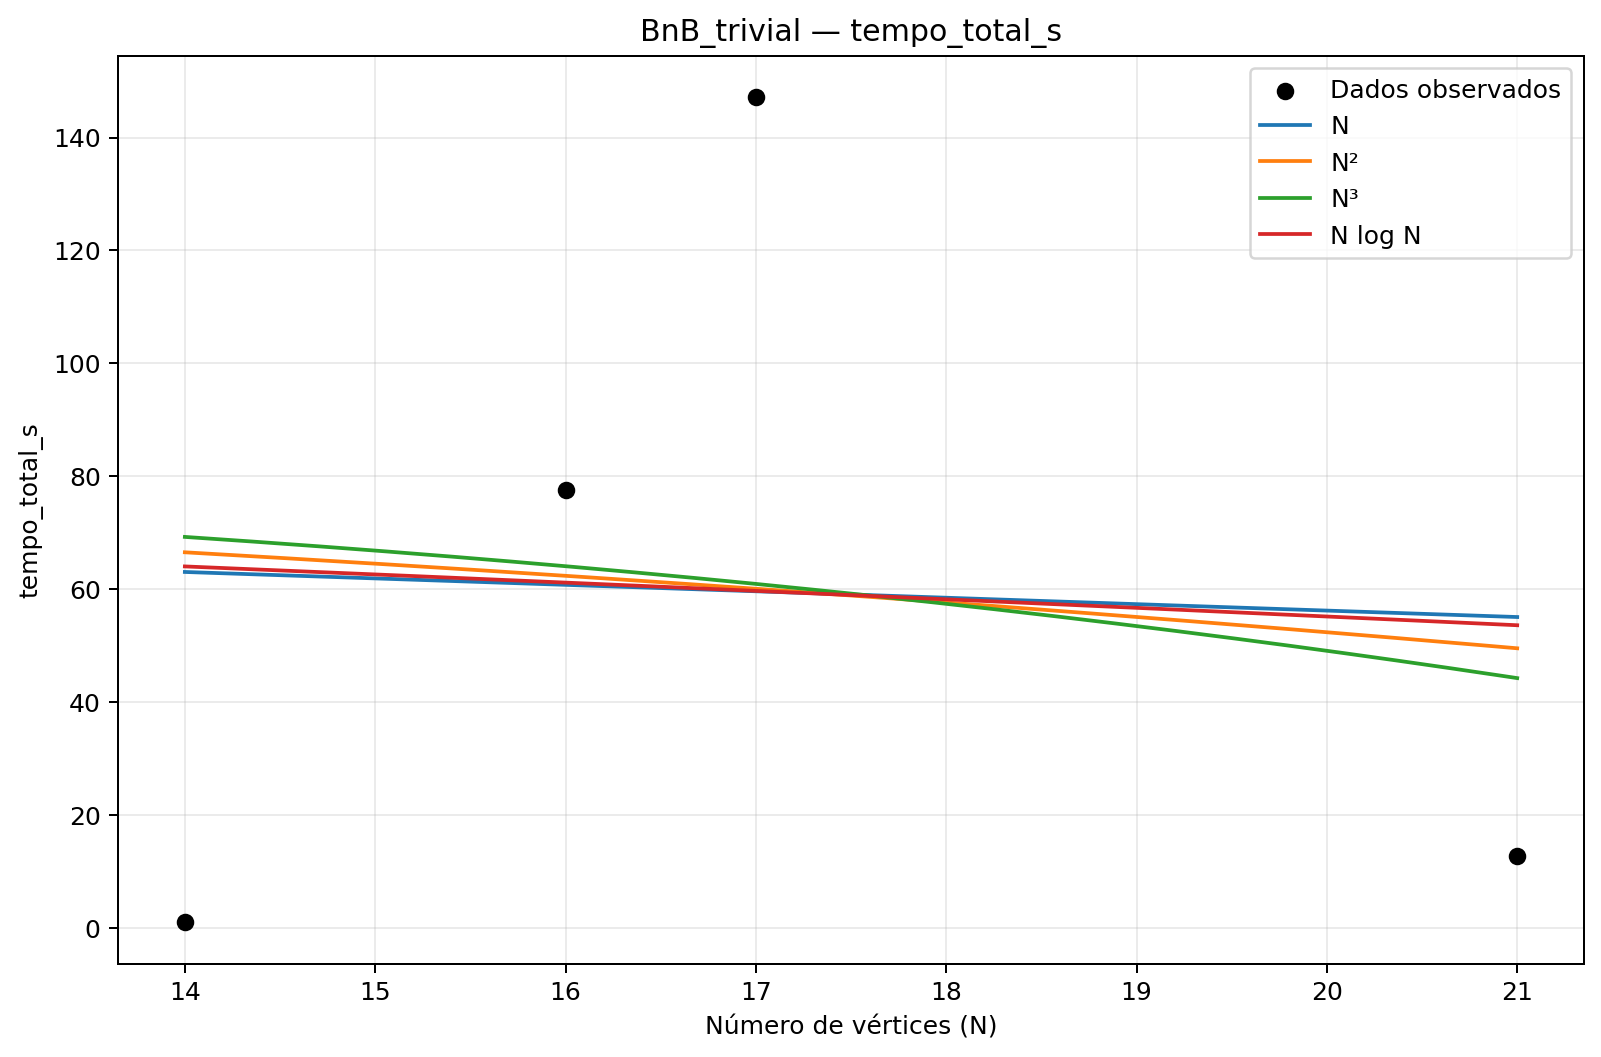
\includegraphics[width=0.48\textwidth]{figuras/regressao_BnB_trivial_tempo_total_s.png}
\hfill
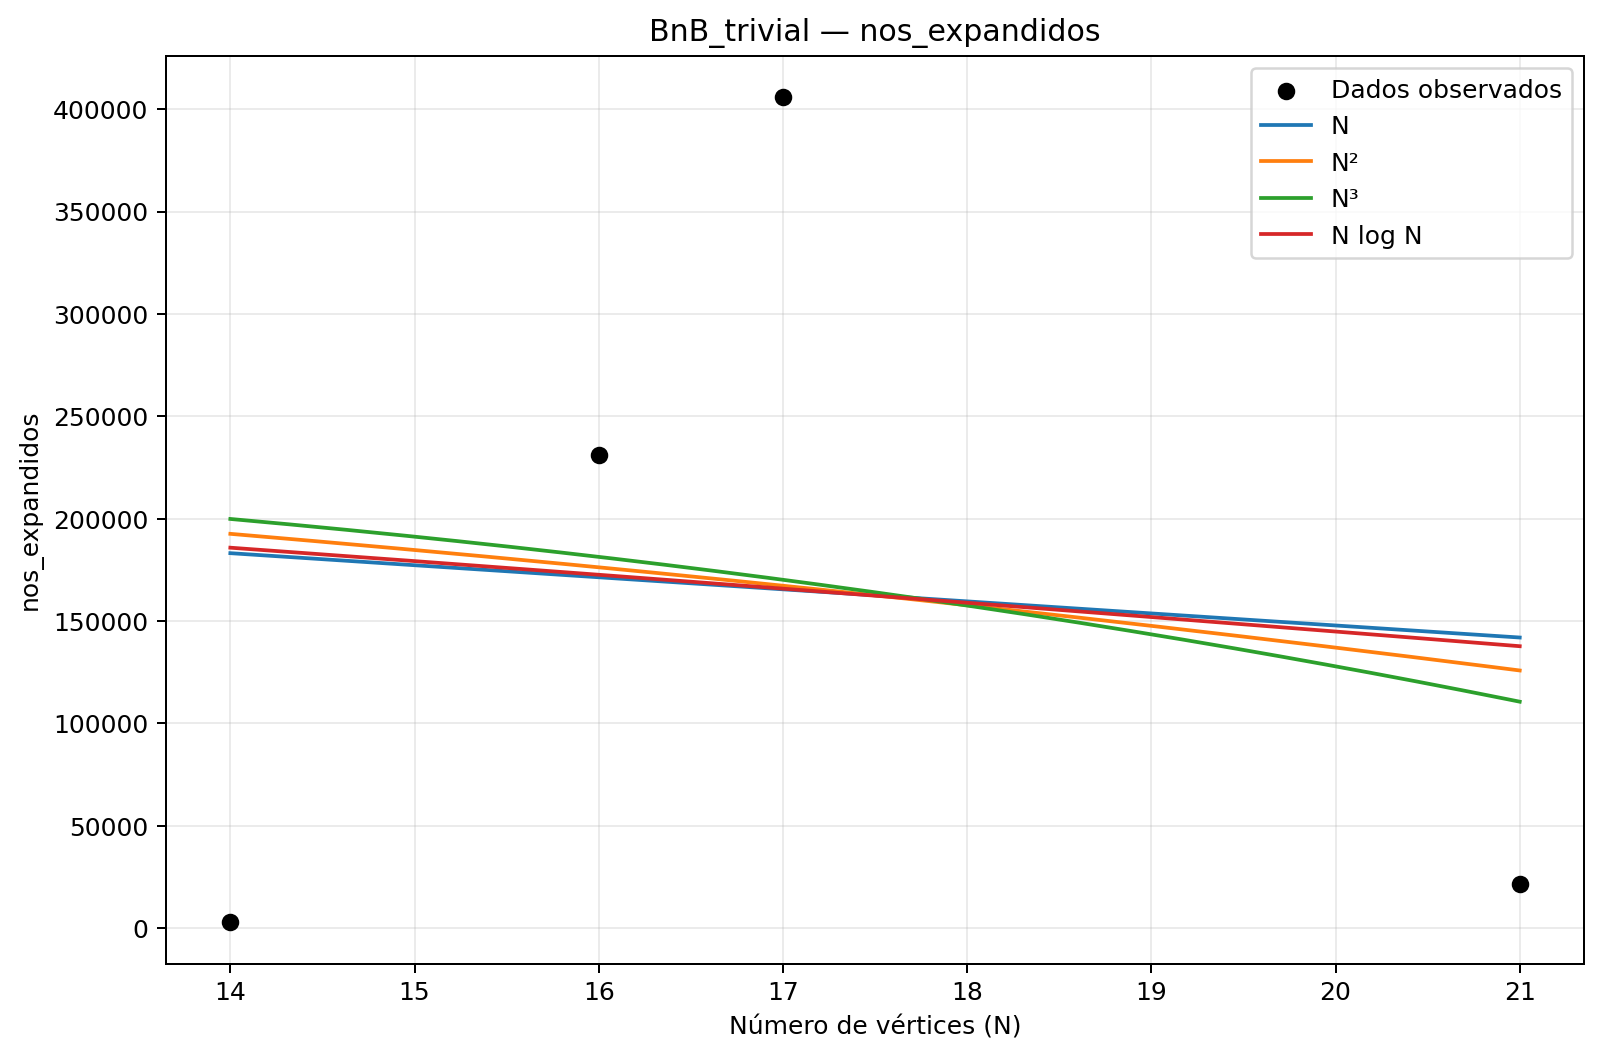
\includegraphics[width=0.48\textwidth]{figuras/regressao_BnB_trivial_nos_expandidos.png}
\caption{Tempo total (esquerda) e nós expandidos (direita) do B\&B (\texttt{trivial}) em função de $N$ para as $4$ instâncias concluídas. Instâncias com $N \ge 22$ sofreram censura por \textit{timeout} e não integram o ajuste.}
\label{fig:reg_bnb}
\end{figure}

\begin{figure}[ht]
\centering
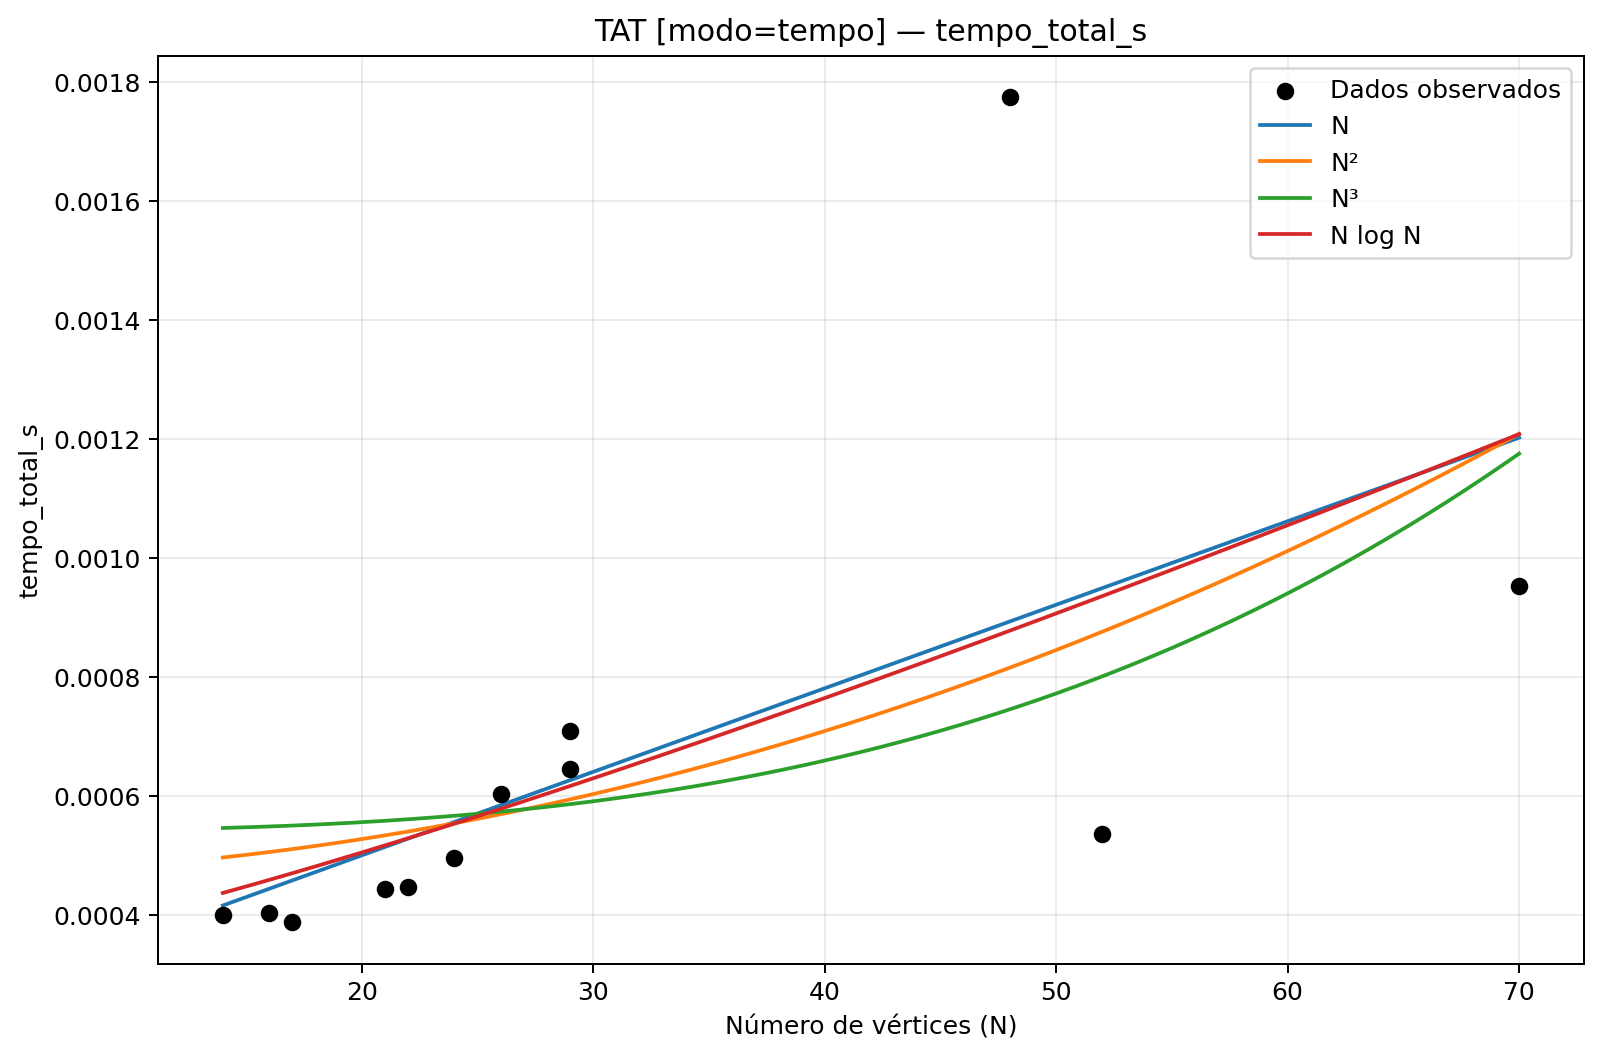
\includegraphics[width=0.48\textwidth]{figuras/regressao_TAT_tempo.png}
\hfill
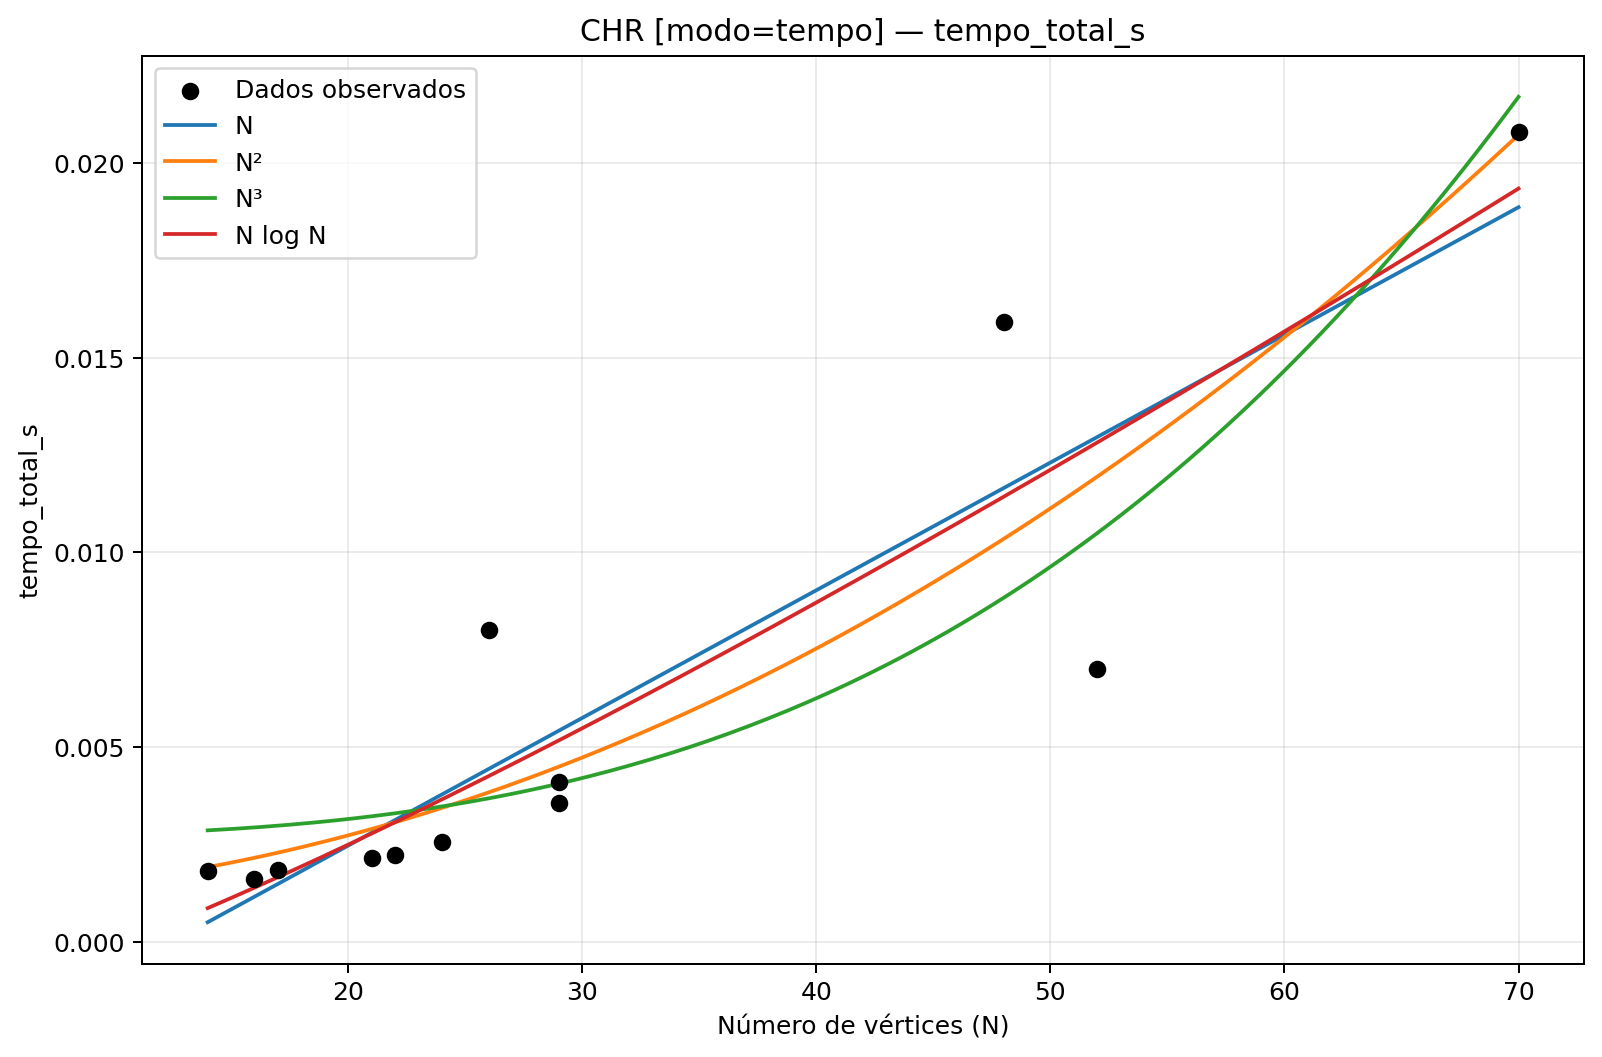
\includegraphics[width=0.48\textwidth]{figuras/regressao_CHR_tempo.png}
\caption{Ajustes empíricos do tempo total de execução em função de $N$ para Twice-around-the-tree (esquerda) e Christofides (direita) sobre as $12$ instâncias.}
\label{fig:reg_aprox}
\end{figure}

\subsection{Custo por Nó e Efeito das Estratégias de Warm-Start}

A Tabela~\ref{tab:custo_no} reporta a mediana do tempo médio despendido por nó expandido nas instâncias concluídas no modo tempo. Observa-se notável estabilidade entre as cinco estratégias: o custo mediano de busca por nó situa-se entre $359{,}71\text{ }\mu\text{s}$ (\texttt{TAT}) e $374{,}91\text{ }\mu\text{s}$ (\texttt{CHR}), praticamente idêntico ao custo total por nó, uma vez que o tempo da heurística inicial é inferior a $0{,}05\text{ s}$ em todas as instâncias. Como o processamento individual de cada estado possui custo quase invariante, o tempo total de resolução do B\&B é determinado essencialmente pelo tamanho da árvore explorada.

\begin{table}[ht]
\centering
\caption{Mediana do custo de processamento por nó expandido ($\mu\text{s}$) e número de instâncias concluídas por estratégia de \textit{warm-start}.}
\label{tab:custo_no}
\small
\begin{tabular}{lccc}
\toprule
\textbf{Estratégia} & \textbf{Custo Total / Nó ($\mu\text{s}$)} & \textbf{Custo Busca / Nó ($\mu\text{s}$)} & \textbf{Instâncias Concluídas} \\
\midrule
\texttt{trivial} & 372,07 & 372,07 & 4 \\
\texttt{vizinho} & 367,60 & 367,59 & 4 \\
\texttt{fecho}   & 363,03 & 362,93 & 2 \\
\texttt{TAT}     & 359,77 & 359,71 & 4 \\
\texttt{CHR}     & 375,21 & 374,91 & 4 \\
\bottomrule
\end{tabular}
\end{table}

Para avaliar o impacto real das heurísticas de inicialização sobre a poda sem enviesar a análise pela diferença de cobertura entre estratégias, a Tabela~\ref{tab:warmstart_pareado} apresenta a comparação estritamente pareada em relação à linha de base \texttt{trivial}, considerando apenas os pares concluídos.

\begin{table}[ht]
\centering
\caption{Comparação pareada de nós expandidos e redução percentual em relação à estratégia \texttt{trivial} nas instâncias concluídas.}
\label{tab:warmstart_pareado}
\small
\begin{tabular}{lcrrrrr}
\toprule
\textbf{Instância} & \textbf{$N$} & \textbf{Nós (\texttt{trivial})} & \textbf{\texttt{vizinho}} & \textbf{\texttt{fecho}} & \textbf{\texttt{TAT}} & \textbf{\texttt{CHR}} \\
\midrule
\texttt{burma14}   & 14 & 2.863   & $0{,}00\%$ & $30{,}63\%$ & $0{,}00\%$ & $15{,}68\%$ \\
\texttt{ulysses16} & 16 & 231.317 & $0{,}00\%$ & $0{,}02\%$  & $0{,}00\%$ & $0{,}01\%$  \\
\texttt{gr17}      & 17 & 406.037 & $0{,}08\%$ & ---         & $0{,}01\%$ & $0{,}08\%$  \\
\texttt{gr21}      & 21 & 21.715  & $0{,}01\%$ & ---         & $0{,}00\%$ & $1{,}41\%$  \\
\bottomrule
\end{tabular}
\end{table}

Os resultados evidenciam que o \textit{warm-start} só reduz efetivamente o espaço de busca quando fornece um limitante superior inicial (UB) estritamente menor do que o custo dos primeiros circuitos hamiltonianos completos alcançados naturalmente pela busca em profundidade (DFS). Na instância \texttt{burma14}, o primeiro circuito completo encontrado pela DFS possui custo $3556$: como os limitantes iniciais fornecidos por \texttt{trivial} ($4562$), \texttt{vizinho} ($4048$) e \texttt{TAT} ($4003$) superam esse patamar, as três estratégias percorrem exatamente os mesmos $2.863$ nós. Em contraste, o algoritmo de Christofides fornece $\text{UB} = 3448$, reduzindo os nós expandidos em $15{,}68\%$ ($2.414$ nós) e o tempo total de $1{,}09\text{ s}$ para $0{,}93\text{ s}$. A inserção pelo fecho convexo alcança redução de $30{,}63\%$ em \texttt{burma14} ($1.986$ nós; $0{,}79\text{ s}$), mas o ganho não se sustenta em \texttt{ulysses16} ($0{,}02\%$), além de não ser aplicável às matrizes \texttt{EXPLICIT}. Nas demais instâncias concluídas (\texttt{ulysses16}, \texttt{gr17} e \texttt{gr21}), as reduções de nós não ultrapassam $1{,}41\%$, demonstrando que o ordenamento guloso dos filhos por menor limite inferior permite à DFS encontrar boas soluções rapidamente, neutralizando o efeito de inicializações heurísticas moderadas.

\begin{figure}[ht]
\centering
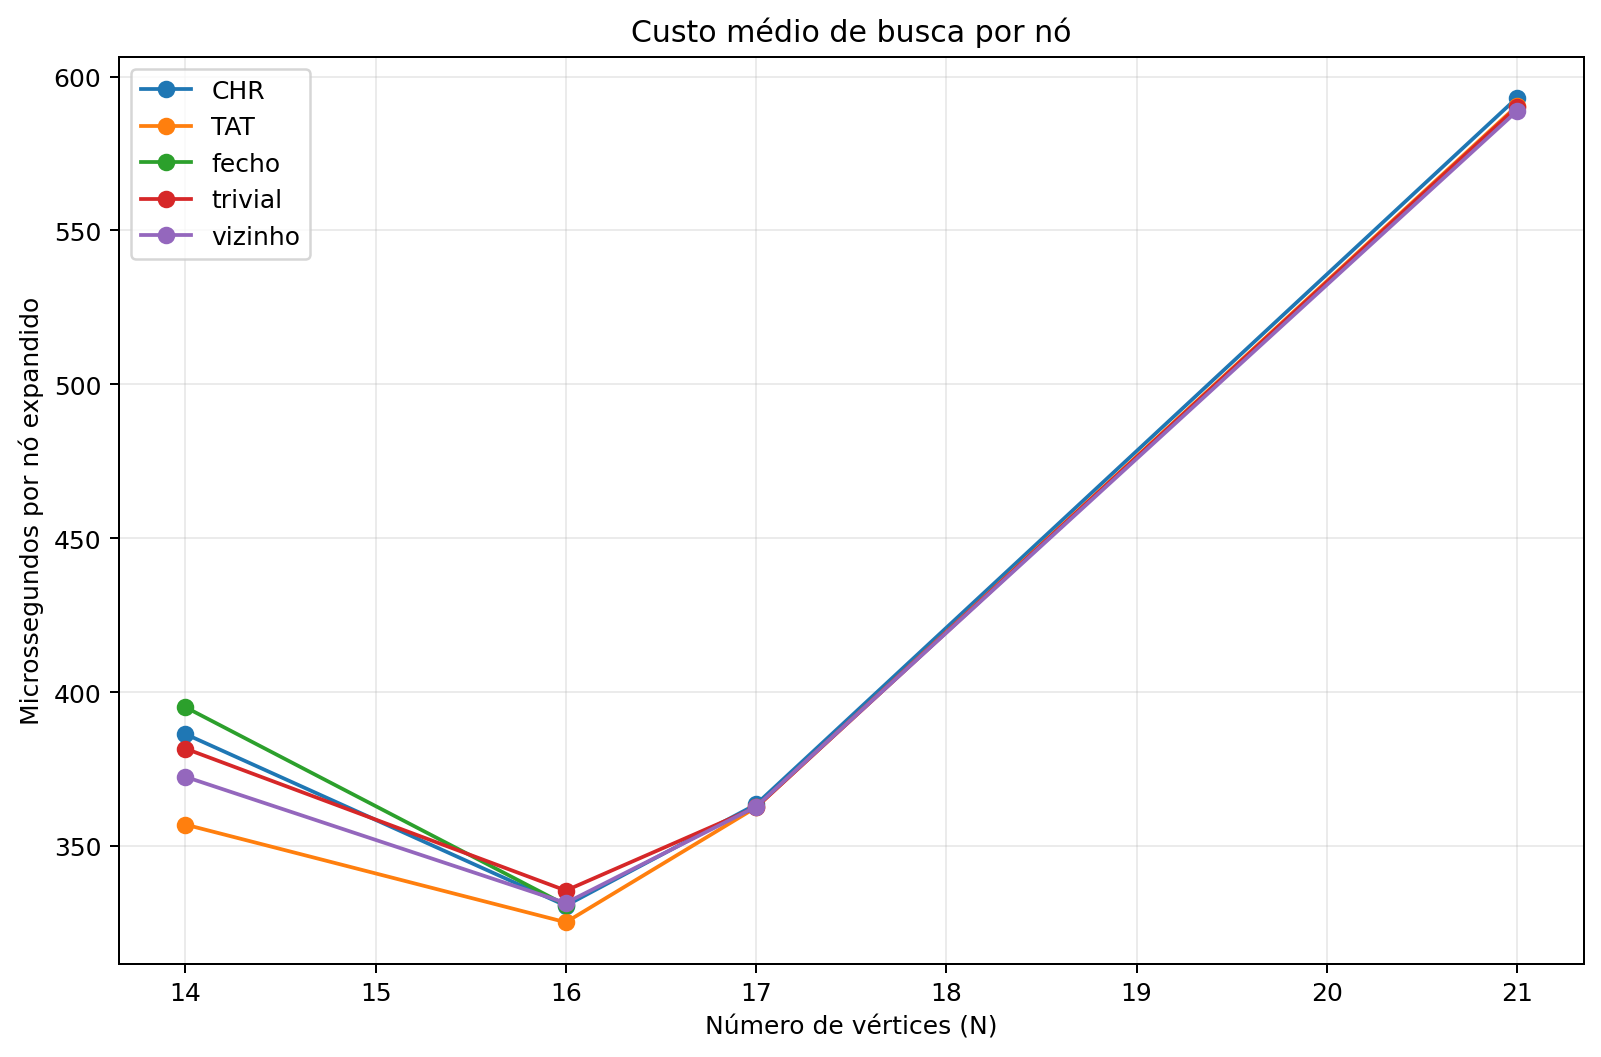
\includegraphics[width=0.48\textwidth]{figuras/custo_por_no.png}
\hfill
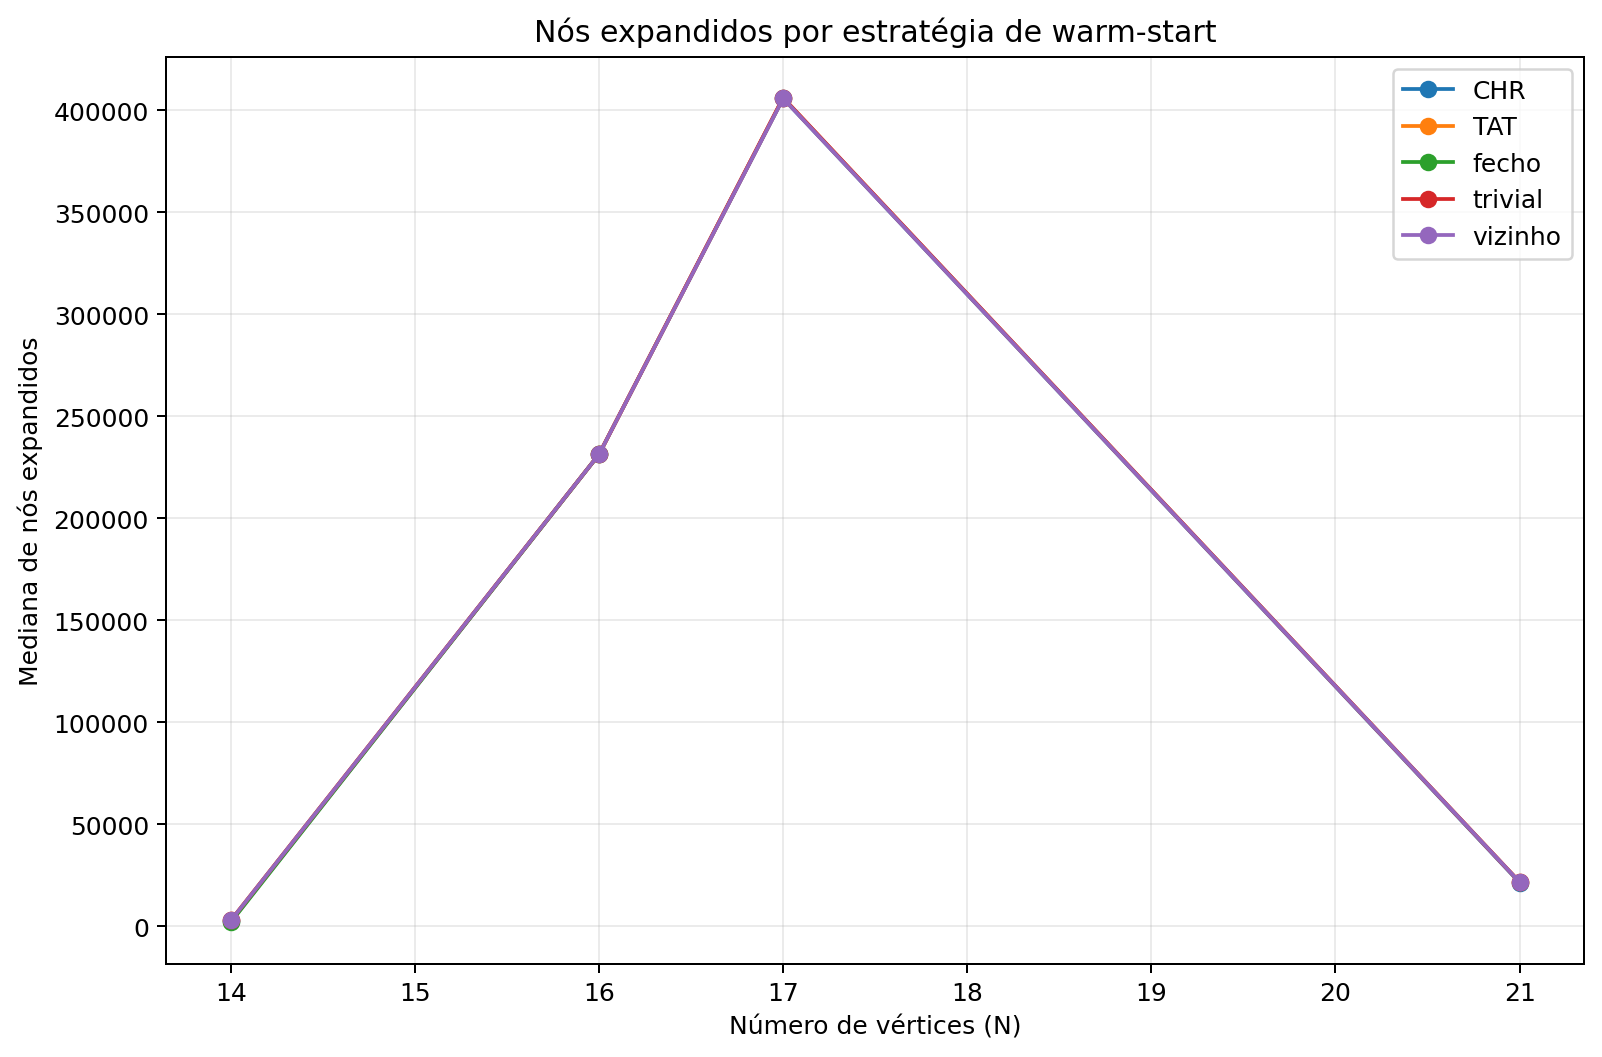
\includegraphics[width=0.48\textwidth]{figuras/nos_expandidos_warmstarts.png}
\caption{Custo médio de busca por nó expandido (esquerda) e total de nós expandidos (direita) por estratégia de \textit{warm-start} nas instâncias concluídas.}
\label{fig:warmstart}
\end{figure}

\subsection{Qualidade e Desempenho dos Algoritmos Aproximativos}

A Tabela~\ref{tab:qualidade_aprox} consolida o \textit{gap} relativo ($\text{custo}/\text{OPT} - 1$) e o tempo mediano de execução de TAT e CHR sobre todas as $12$ instâncias. Como ambas as heurísticas são determinísticas sobre a matriz $D$, os \textit{gaps} são idênticos entre todas as repetições e modos.

\begin{table}[ht]
\centering
\caption{\textit{Gap} relativo e tempo mediano de execução (modo tempo) das heurísticas TAT e CHR nas $12$ instâncias.}
\label{tab:qualidade_aprox}
\small
\begin{tabular}{lccccc}
\toprule
\textbf{Instância} & \textbf{$N$} & \textbf{Tipo} & \textbf{\textit{Gap} TAT} & \textbf{\textit{Gap} CHR} & \textbf{Tempo TAT / CHR (ms)} \\
\midrule
\texttt{burma14}   & 14 & \texttt{GEO}      & 0,2046 & 0,0376 & 0,4 / 1,8 \\
\texttt{ulysses16} & 16 & \texttt{GEO}      & 0,1354 & 0,0184 & 0,4 / 1,6 \\
\texttt{gr17}      & 17 & \texttt{EXPLICIT} & 0,1281 & 0,0504 & 0,4 / 1,8 \\
\texttt{gr21}      & 21 & \texttt{EXPLICIT} & 0,3809 & 0,0277 & 0,4 / 2,1 \\
\texttt{ulysses22} & 22 & \texttt{GEO}      & 0,1847 & 0,0620 & 0,4 / 2,2 \\
\texttt{gr24}      & 24 & \texttt{EXPLICIT} & 0,2901 & 0,1061 & 0,5 / 2,6 \\
\texttt{fri26}     & 26 & \texttt{EXPLICIT} & 0,2124 & 0,0416 & 0,6 / 8,0 \\
\texttt{bayg29}    & 29 & \texttt{EXPLICIT} & 0,3621 & 0,0789 & 0,7 / 3,6 \\
\texttt{bays29}    & 29 & \texttt{EXPLICIT} & 0,3252 & 0,1099 & 0,6 / 4,1 \\
\texttt{att48}     & 48 & \texttt{ATT}      & 0,3103 & 0,0837 & 1,8 / 15,9 \\
\texttt{berlin52}  & 52 & \texttt{EUC\_2D}  & 0,3792 & 0,0911 & 0,5 / 7,0 \\
\texttt{st70}      & 70 & \texttt{EUC\_2D}  & 0,2948 & 0,1096 & 1,0 / 20,8 \\
\bottomrule
\end{tabular}
\end{table}

O algoritmo de Christofides superou o TAT em qualidade em $100\%$ das instâncias avaliadas, apresentando \textit{gap} mediano global de $7{,}05\%$ (mínimo de $1{,}84\%$ em \texttt{ulysses16} e máximo de $10{,}99\%$ em \texttt{bays29}), contra \textit{gap} mediano de $29{,}25\%$ do TAT (mínimo de $12{,}81\%$ em \texttt{gr17} e máximo de $38{,}09\%$ em \texttt{gr21}). Em contrapartida, o TAT mostrou-se sistematicamente mais rápido, concluindo a maior instância (\texttt{st70}) em $1{,}0\text{ ms}$, frente a $20{,}8\text{ ms}$ do CHR. Ambos os algoritmos respeitaram os fatores teóricos de pior caso ($2$ e $1{,}5$) em todas as instâncias, inclusive naquelas que violam a desigualdade triangular após o arredondamento inteiro; contudo, dado o tamanho reduzido da amostra ($5$ instâncias métricas e $7$ não métricas), não se pode estabelecer uma inferência estatística comparativa entre esses dois subgrupos.

\begin{figure}[ht]
\centering
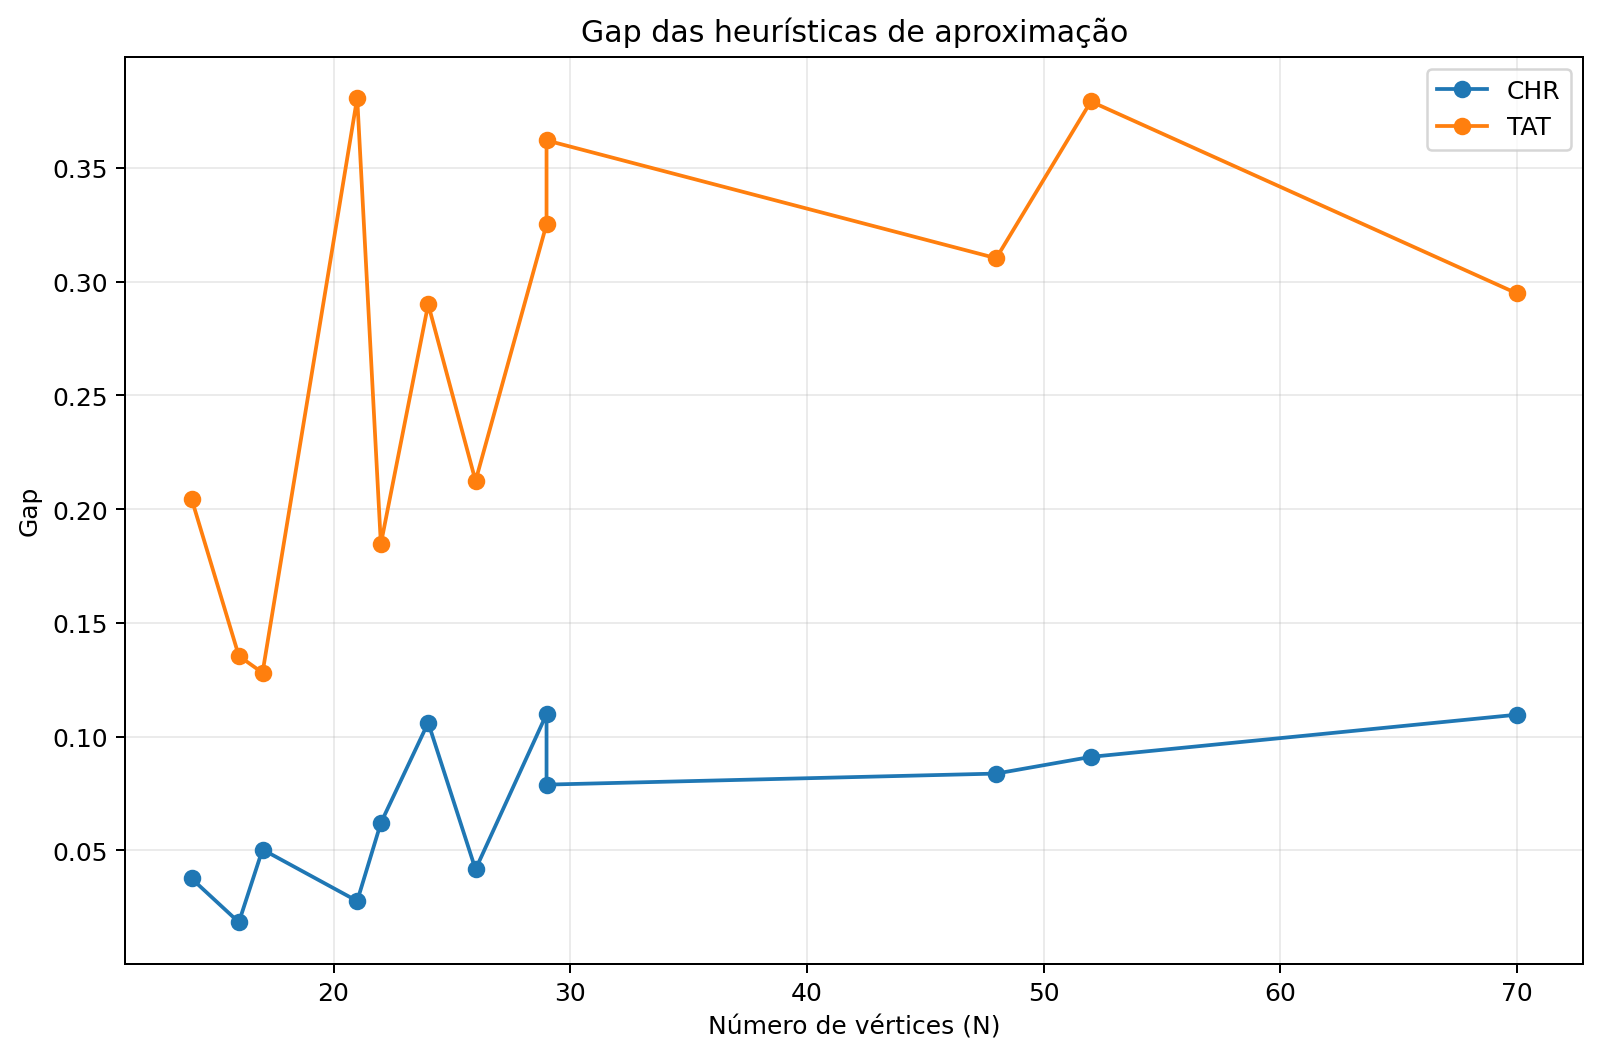
\includegraphics[width=0.48\textwidth]{figuras/gap_aproximacao.png}
\hfill
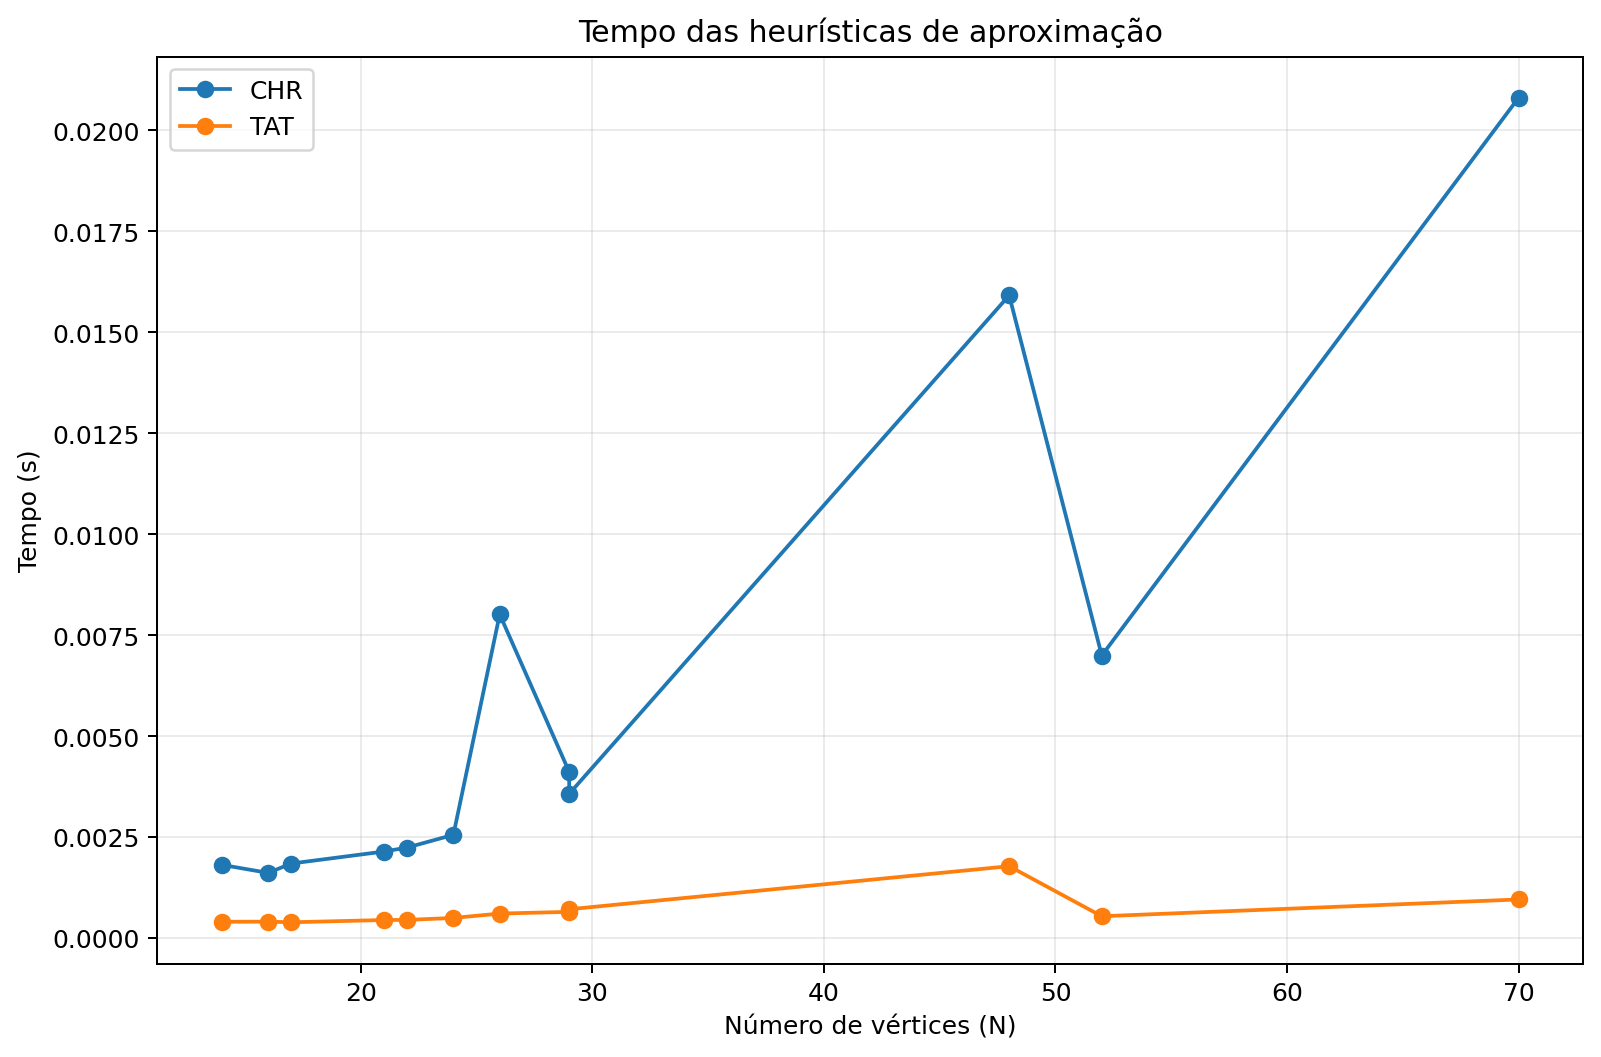
\includegraphics[width=0.48\textwidth]{figuras/tempo_aproximacao.png}
\caption{Comparação do \textit{gap} relativo (esquerda) e do tempo mediano de execução (direita) entre TAT e CHR ao longo das $12$ instâncias.}
\label{fig:aprox_qualidade}
\end{figure}

\subsection{Análise de Sensibilidade às Características Geométricas}

Para investigar a relação entre propriedades estruturais das instâncias e o erro de aproximação, calcularam-se correlações de Spearman ($\rho$) com $p$-valores bilaterais exatos por permutação ($9.999$ reamostragens) entre as oito métricas extraídas em \texttt{features.py} e o \textit{gap} individual de cada heurística (Tabela~\ref{tab:spearman}). As $6$ instâncias \texttt{EXPLICIT} foram excluídas por não possuírem coordenadas, restringindo a amostra a $n = 6$ instâncias (\texttt{burma14}, \texttt{ulysses16}, \texttt{ulysses22}, \texttt{att48}, \texttt{berlin52} e \texttt{st70}). Optou-se pela análise bivariada não paramétrica em vez de regressão múltipla ou árvores de decisão porque, com $n = 6$ observações e $8$ preditores, modelos multivariados sofreriam grande sobreajuste.

\begin{table}[ht]
\centering
\caption{Correlação de Spearman ($\rho$) e $p$-valor bilateral por permutação entre características geométricas e \textit{gap} ($n = 6$ instâncias com coordenadas).}
\label{tab:spearman}
\small
\begin{tabular}{lcccc}
\toprule
\textbf{Característica (\textit{Feature})} & \textbf{$\rho$ (TAT)} & \textbf{$p$-valor (TAT)} & \textbf{$\rho$ (CHR)} & \textbf{$p$-valor (CHR)} \\
\midrule
Razão de aspecto                 & $-0{,}8117$ & $0{,}0728$ & $-0{,}8986$ & $0{,}0268$ \\
Proporção no fecho convexo       & $-0{,}7714$ & $0{,}1104$ & $-1{,}0000$ & $0{,}0014$ \\
Entropia espacial                & $+0{,}7714$ & $0{,}1112$ & $+0{,}8857$ & $0{,}0332$ \\
Densidade de \textit{clustering} & $-0{,}9429$ & $0{,}0166$ & $-0{,}8286$ & $0{,}0608$ \\
Grau máximo da MST               & $+0{,}2928$ & $0{,}7012$ & $+0{,}2928$ & $0{,}6872$ \\
CV da distância ao vizinho prox. & $-0{,}5429$ & $0{,}3052$ & $-0{,}6000$ & $0{,}2412$ \\
Distância média                  & $+0{,}7143$ & $0{,}1394$ & $+0{,}6000$ & $0{,}2432$ \\
Desvio-padrão das distâncias     & $+0{,}7143$ & $0{,}1394$ & $+0{,}6000$ & $0{,}2432$ \\
\bottomrule
\end{tabular}
\end{table}

Na amostra observada, o \textit{gap} do Christofides apresenta correlação negativa perfeita com a proporção de vértices no fecho convexo ($\rho = -1{,}0000$, $p = 0{,}0014$). Geometricamente, instâncias com maior fração de pontos na envoltória convexa exigem menos desvios internos para fechar o ciclo hamiltoniano, favorecendo a etapa de emparelhamento e atalhos. Para o TAT, sugere-se que são vistos maiores \textit{gaps} em distribuições espacialmente mais dispersas (maior entropia). Ressalta-se, contudo, que quatro das seis instâncias analisadas pertencem aos tipos \texttt{GEO} e \texttt{ATT} (cujas métricas reais não são euclidianas no plano), e a colinearidade entre as características impõe cautela na interpretação: esses coeficientes representam indícios exploratórios de associação, e não relações de causalidade.

\subsection{Profiling de Subrotinas e Gargalos Computacionais}

A decomposição do tempo por subrotina revela gargalos estruturais distintos entre as abordagens avaliadas:
\begin{itemize}
    \item \textbf{Twice-around-the-tree (etapas disjuntas):} A construção da Árvore Geradora Mínima (\texttt{prim\_mst}) concentra entre $88{,}47\%$ (\texttt{ulysses16}) e $95{,}55\%$ (\texttt{att48}) do tempo total de execução. As demais subrotinas somam menos de $12\%$ em todas as instâncias (\texttt{atalhos} e \texttt{validar\_e\_custo} respondem por cerca de $1{,}2\%$ a $2{,}8\%$ cada, e \texttt{grau\_mst} por aproximadamente $0{,}5\%$ a $1{,}4\%$).
    \item \textbf{Christofides (etapas disjuntas):} O cálculo do emparelhamento perfeito de custo mínimo (\texttt{emparelhamento} via NetworkX) domina amplamente o custo computacional, variando de $74{,}04\%$ do tempo total na menor instância (\texttt{burma14}) até $95{,}10\%$ em \texttt{att48} e $94{,}78\%$ em \texttt{st70}. A participação da MST (\texttt{prim\_mst}) cai proporcionalmente de $20{,}35\%$ para $3{,}92\%$ à medida que $N$ cresce, enquanto \texttt{euler}, \texttt{atalhos}, \texttt{grau\_mst} e \texttt{validar\_e\_custo} somam menos de $3\%$. Confirma-se, portanto, que o algoritmo de Blossom utilizado no emparelhamento constitui o principal gargalo prático do CHR.
    \item \textbf{Branch-and-Bound (subrotinas aninhadas):} Como a hierarquia de chamadas do B\&B é aninhada ($\texttt{matriz\_reducao} \subset \texttt{calculo\_lb} \subset \texttt{expansao\_no} \subset \texttt{busca\_total}$), suas frações não são aditivas e são expressas em relação ao tempo interno de \texttt{busca\_total}. Nas instâncias de médio e grande porte, \texttt{expansao\_no} absorve cerca de $99{,}0\%$ a $99{,}7\%$ do tempo de busca, \texttt{calculo\_lb} representa entre $93{,}9\%$ e $96{,}1\%$, e \texttt{matriz\_reducao} responde isoladamente por $58{,}8\%$ a $67{,}3\%$ do tempo total. A rotina de \texttt{warmstart} consome menos de $0{,}2\%$ em todos os cenários. Esses números demonstram que a cópia integral e a redução linha-coluna da matriz $N \times N$ a cada nó gerado constituem o gargalo dominante da busca exata.
\end{itemize}

\subsection{Auditoria de Memória e Violações da Desigualdade Triangular}
\label{sec:violacoes}

\paragraph{Consumo de Memória.} O monitoramento via \texttt{tracemalloc} captura exclusivamente objetos alocados pelo interpretador Python dentro do escopo instrumentado, não contabilizando buffers nativos pré-alocados fora das subrotinas ou o RSS total do processo. Consequentemente, os picos registrados para TAT e CHR ($0{,}004\text{ MB}$ a $0{,}06\text{ MB}$) subestimam a pegada real da matriz $D$ ($\mathcal{O}(N^2)$) e devem ser interpretados apenas como o custo das estruturas auxiliares (pilhas, listas de adjacência e grafos do NetworkX). No B\&B, o pico de memória cresce monotonicamente com a profundidade e o tamanho das submatrizes empilhadas nas instâncias concluídas (de $0{,}0697\text{ MB}$ em \texttt{burma14} a $0{,}2130\text{ MB}$ em \texttt{gr21} para \texttt{trivial}), enquanto $36$ execuções no modo memória atingiram o limite de tempo devido à sobrecarga de rastreamento do \texttt{tracemalloc}.

\paragraph{Desigualdade Triangular.} A auditoria métrica separou as violações na matriz de coordenadas em ponto flutuante (\texttt{violacoes\_reais}, aplicável às $2$ instâncias \texttt{EUC\_2D}) das violações na matriz inteira $D$ efetivamente consumida pelos algoritmos (\texttt{violacoes\_arredondadas}, avaliadas nas $12$ instâncias). Nas duas instâncias euclidianas (\texttt{berlin52} e \texttt{st70}), não há nenhuma violação em ponto flutuante ($\texttt{violacoes\_reais} = 0$), mas o arredondamento ao inteiro mais próximo (\texttt{nint}) introduz, respectivamente, $160$ e $758$ triplas que violam a desigualdade triangular. Das $12$ instâncias totais, $7$ apresentam violações na matriz inteira ($5$ \texttt{EXPLICIT} e $2$ \texttt{EUC\_2D}) e $5$ mantêm a propriedade métrica intacta. Esse achado comprova que instâncias geometricamente euclidianas da TSPLIB tornam-se tecnicamente não métricas após a discretização padrão da biblioteca, embora, na prática, ambos os algoritmos aproximativos tenham permanecido bem abaixo dos limitantes teóricos de pior caso.

\section{Conclusões}

Este trabalho investigou o desempenho empírico, a estrutura de custos por subrotina e os limites práticos de um resolvedor exato baseado em \textit{Branch-and-Bound} (B\&B) frente aos algoritmos aproximativos \textit{Twice-around-the-tree} (TAT) e Christofides (CHR) sobre $12$ instâncias da TSPLIB.

Os resultados experimentais sustentam quatro conclusões principais:
\begin{enumerate}
    \item \textbf{Compromisso entre otimalidade, tempo e escalabilidade:} Enquanto o B\&B garantiu a solução ótima exata nas quatro instâncias de menor porte ($N \le 21$), todas as instâncias com $N \ge 22$ excederam o limite de $1800\text{ s}$ ($91$ ocorrências de \textit{timeout} no total), revelando que a barreira prática da busca exata com redução matricial em Python se manifesta ainda dentro da faixa principal de tamanhos ($N \le 40$). Em contrapartida, TAT e CHR concluíram $100\%$ das execuções em no máximo $20{,}8\text{ ms}$, com o algoritmo de Christofides entregando soluções substancialmente superiores (\textit{gap} mediano de $7{,}05\%$ contra $29{,}25\%$ do TAT).
    \item \textbf{Condição de efetividade do \textit{warm-start}:} Como o custo de processamento por nó expandido manteve-se praticamente invariante entre as estratégias ($\approx 360$ a $375\text{ }\mu\text{s}$), a inicialização heurística só reduz o tempo total quando fornece um limitante superior inicial estritamente melhor que os primeiros circuitos completos encontrados naturalmente pela busca em profundidade (DFS). Na instância \texttt{burma14}, o CHR reduziu os nós expandidos em $15{,}68\%$ e o fecho convexo em $30{,}63\%$, mas nas demais instâncias concluídas as reduções foram marginais ($\le 1{,}41\%$), pois o ordenamento guloso dos filhos por menor limite inferior permitiu à DFS encontrar boas soluções incumbentes rapidamente.
    \item \textbf{Gargalos algorítmicos identificados pelo \textit{profiling}:} A instrumentação em nível de subrotina confirmou que os gargalos teóricos dominam o tempo prático: no TAT, a construção da MST via Prim responde por $88{,}47\%$ a $95{,}55\%$ do tempo; no CHR, o emparelhamento perfeito mínimo consome de $74{,}04\%$ a $95{,}10\%$ (crescendo com $N$); e no B\&B, a subrotina de redução matricial absorve cerca de $59\%$ a $67\%$ do tempo de busca devido à cópia integral de submatrizes $N \times N$ a cada expansão.
    \item \textbf{Impacto da discretização na propriedade métrica e associação geométrica:} A auditoria demonstrou que o arredondamento inteiro padrão da TSPLIB (\texttt{nint}) introduz violações da desigualdade triangular mesmo em instâncias puramente euclidianas (\texttt{berlin52} e \texttt{st70}), embora os fatores teóricos de pior caso tenham sido respeitados empiricamente. Na análise exploratória de sensibilidade ($n=6$), observou-se forte correlação negativa entre o \textit{gap} do CHR e a proporção de vértices no fecho convexo ($\rho = -1{,}0000$, $p = 0{,}0014$).
\end{enumerate}

\paragraph{Limitações e Trabalhos Futuros.} As conclusões deste estudo devem ser interpretadas à luz de suas restrições metodológicas: (i) a amostra limita-se a $12$ instâncias da TSPLIB (com apenas $6$ possuindo coordenadas espaciais, das quais $4$ são não euclidianas dos tipos \texttt{GEO} e \texttt{ATT}), de modo que as regressões empíricas e correlações de Spearman possuem caráter exploratório e não demonstram classes de complexidade assintótica nem causalidade; (ii) repetições experimentais quantificam a variabilidade operacional, mas não aumentam o número de instâncias independentes; (iii) a censura por \textit{timeout} no B\&B exclui as instâncias mais difíceis das curvas ajustadas; (iv) o módulo \texttt{tracemalloc} contabiliza exclusivamente alocações gerenciadas pelo interpretador Python dentro das subrotinas instrumentadas, subestimando a pegada de memória nativa da matriz $D$; e (v) as execuções dos modos de tempo e memória ocorreram em de \textit{hardwares} distintos, impedindo comparações cruzadas diretas entre esses modos. Como trabalhos futuros, recomenda-se substituir a cópia integral de matrizes no B\&B por estruturas incrementais de redução ou programação dinâmica, além de incorporar métricas de RSS do sistema operacional para auditar o consumo total de memória.

\bibliographystyle{sbc}

\end{document}